
RethinkDB es...


\subsection{Sharding}

La consigna del TP pide experimentar con sharding. Para esto utilizamos la tabla que contiene a todos los árbitros, dado que es la más fácil de generar valores aleatorios para insertar.

Inicializamos la tabla con 1 shard y \textasciitilde 100 valores.

\begin{figure}[H]
 \centering
 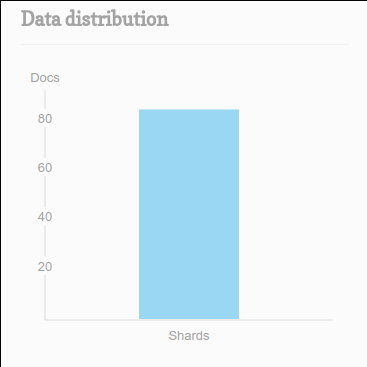
\includegraphics[width=2.5in]{sharding/img/1shard.png}
 \caption{1 shard con \textasciitilde 100 valores}
 \label{fig:1shard}
\end{figure}

Luego pasamos a 2 shards, manteniendo los \textasciitilde 100 valores.

\begin{figure}[H]
 \centering
 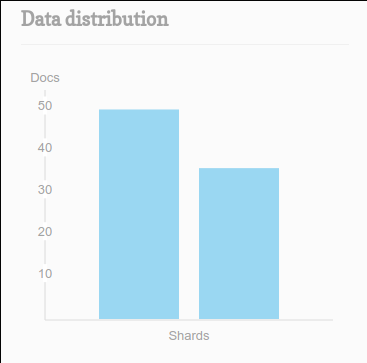
\includegraphics[width=2.5in]{sharding/img/2shard.png}
 \caption{2 shards con \textasciitilde 100 valores}
 \label{fig:2shard}
\end{figure}

Finalmente pasamos a 3 shards, manteniendo los \textasciitilde 100 valores.

\begin{figure}[H]
 \centering
 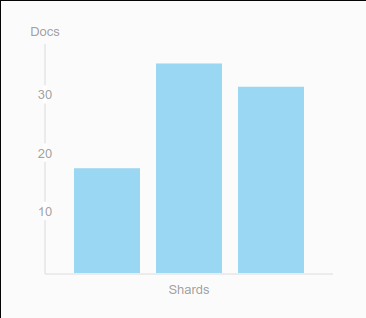
\includegraphics[width=2.5in]{sharding/img/3shard100.png}
 \caption{3 shards con \textasciitilde 100 valores}
 \label{fig:3shard100}
\end{figure}

Luego empezamos a aumentar la cantidad de documentos de la tabla, de a cientos o a más. Graficamos las siguientes cantidades: 100, 200, 300, 400, 700, 1000, 1500, 2000, 4000. Se puede apreciar que la distrubución que vemos cuando hay sólo 100 documentos perdura a lo largo de todas las inserciones.

\begin{figure}[H]
\centering
\begin{tabular}{|l | l | l | l|}
  \hline
  \# Documentos & Shard 1 & Shard 2 & Shard 3 \\
  \hline
  100           & 18  & 36  & 32 \\
  200           & 50  & 80  & 70 \\
  300           & 65  & 115 & 95 \\
  400           & 84  & 170 & 115 \\
  700           & 145 & 265 & 235 \\
  1000          & 185 & 395 & 306 \\
  1500          & 265 & 563 & 480 \\
  2000          & 405 & 747 & 700 \\
  4000          & 718 & 1595 & 1384 \\
  \hline
\end{tabular}
 \caption{Tabla de como avanza la distribución de documentos por shard cuando insertamos más documentos. Notar que todos los valores, que fueron extraídos de la interfaz gráfica de RethinkDB, son aproximados, RethinkDB no garantiza exactitud en estas estadísticas.}
 \label{fig:shardstabla}
\end{figure}


\begin{figure}[H]
 \centering
 \includegraphics[width=5in]{shards.pdf}
 \caption{Gráfico de la tabla anterior}
 \label{fig:shardslinea}
\end{figure}


Por ejemplo, veamos la distribución con \textasciitilde 4000 documentos:
\begin{figure}[H]
 \centering
 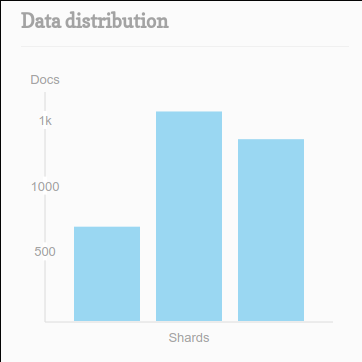
\includegraphics[width=2.5in]{sharding/img/3shard4000.png}
 \caption{3 shards con \textasciitilde 4000 valores}
 \label{fig:3shard4000}
\end{figure}
